\section{Motivation} 

%% Before beginning, let's explain what reinforcement learning is
Reinforcement Learning is a method of learning that maps situations to
actions in order to maximize its rewards
\cite{sutton2018reinforcement}. Rewards are numerical values
associated to a state and action. Precisely, one defines a reward
function $R : (S \times A) \rightarrow \mathbb{R}$ where $S$ defines the state space and $A$ the action space.
This function is equivalent to $R' : S \rightarrow mathbb{R}$ where the queried state is the one resulting from a given (state, action) pair. 
Those can be used interchangeably. More precisely, in the case we describe, the state refers to the current configuration
of the environment and the action refers to the action chosen by the RL agent. By defining this reward function and the scenario of the problem the agent is trying to solve, 
reinforcement learning has the advantage of not requiring a prior dataset. Indeed, the agent is not told what to do, but rather 
learns from the effect of its actions on the environment. 

\begin{figure}[H]
  \centering
  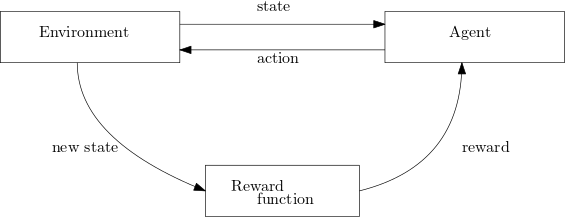
\includegraphics[scale=0.4]{figures/rlroutine.png}
  \caption{Reinforcement Learning Routine}
  \label{fig:rl}
\end{figure}


The diagram in Figure~\ref{fig:rl} is a high-level description of how
an agent using reinforcement learning can be trained.  
%
The upper left box represents the \emph{environment} as seen by the agent
according to its sensors.
%
The current state of the environment is represented as a \emph{state
vector}.
%
At each iteration, the agent will receive the state vector as input,
and needs to choose an \emph{action} to take.
%
Once the action is taken, the environment is updated to the next state
and the agent receives a \emph{reward} as feedback.
%
This reward is a domain dependent function that represents how
``good'' the new state is.
%
The agent's goal is to increase its reward by taking actions that
reach better states each time.
%
The triple (state, action, reward) helps the agent in shaping the
final policy.

%% Reward function is crucial for RL
The reward function is a crucial aspect of the RL algorithm.
%% Here's an example of how it affects training
For instance, consider a game of chess 
where the agent is punished when it loses and rewarded if it wins. The agent is bound to learn how to 
maximize its winnings but it will need to exhaust multiple possible combinations to learn. In this case, 
the training time is not optimal. A better approach would be to also reward it for making a good opening, for instance. 
Another example would be only considering negative rewards. Say we want our agent to escape a maze, and we punish it at every timestep for not escaping. 
If there is a fatality state (\emph{e.g.}, a fire or a black whole), the agent will learn to move towards the fatality state as to cut its negative rewards as soon as possible. 
In conclusion, a good reward function is the first step of optimal learning.
%% Even research says the same! 
By choosing a \emph{refined} reward function, 
we can ensure a faster and more efficient training~\cite{Koenig1996}, possibly with fewer errors. 

\subsection{Reward Shaping}
\label{sec:challenges}

%% Reward shaping is important for a fast and efficient learning
\emph{Reward shaping}~\cite{laud2011} refers to the lack of systematic methods to design a reward
  function that ensures fast and efficient learning~\cite{Koenig1996}. This generation of an appropriate 
reward function for a given problem is still an open challenge~\cite{kober2013}.
%
%% Look at the evidence that shows the importance of it! (examples)
The importance of a reward function for efficient training is shown in~\cite{Koenig1996}.
A sparse reward function defined as a \emph{goal-reward representation} is one where the agent is only rewarded 
for entering a goal state, while a dense reward function is defined as an \emph{action-penalty representation}, precisely, one 
where the agent is penalized for every action it executes. \cite{Koenig1996} shows that a denser reward structure improves performance. 
%
%% That's not all! A good reward function can guide exploration and
%% exploitation as necessary :) 
Moreover, an informed reward function is able to sufficiently deter the exploration of 
undesirable states while encourage the exploitation of desirable ones, continuously adapting to 
acquire knowledge and resolving the conflict when necessary. Precisely, an informed reward function 
can tackle the \emph{exploration vs. exploitation dilemma}, a central challenge in RL~\cite{Kaelbling1996ReinforcementLA}. 
%
%% But when deployed, it can also help in tackling new/unforeseen situations better
In particular, an agent that can continuously acquire knowledge is responding to the uncertainties of the world, where states can never be exhausted. 
This involves an adaptive learned policy that responds to conditions and tasks that were not encountered in the past~\cite{gupta_meta-reinforcement_2018,schweighofer_meta-learning_2003}.
%

%% 'Perfect' reward function would be a native reward
Ideally, rewards would be given by the real-world, i.e. \textit{native rewards}. For instance, recent work investigates dynamically generating a reward 
using a user verbal feedback to the autonomous agent~\cite{gonzalez2010}.
%
%% However, this cannot be applied in practice because most training happens in simulation
%
However, most RL agents can only stay in simulation because the trial-and-error nature of RL prevents any guarantees of safety.
Thus, there exists a need for \textit{shaping rewards} instead.
%
%% As a result, people can only use those 'sparse' reward structure
Unfortunately, due to the lack of systematic methods to build a denser reward function, 
it is common to use a sparse reward function as long as it still guarantees convergence.
